%----------------------------------------------------------------------------------------
%	PACKAGES AND DOCUMENT CONFIGURATIONS
%----------------------------------------------------------------------------------------
\documentclass{article}

\usepackage{graphicx} 	% Required for the inclusion of images
\usepackage{natbib} 	% Required to change bibliography style to APA
\usepackage{amsmath} 	% Required for some math elements 
\usepackage{array}
\usepackage{caption}
\usepackage{subcaption}

\usepackage{xcolor}
\usepackage{listings}
\usepackage{color}		 %red, green, blue, yellow, cyan, magenta, black, white
\usepackage{geometry}
\geometry{
a4paper,
total={170mm,257mm},
left=20mm,
top=20mm,
}
\setlength\parindent{0pt} % Removes all indentation from paragraphs

\definecolor{codegreen}{rgb}{0,0.6,0}
\definecolor{codegray}{rgb}{0.5,0.5,0.5}
\definecolor{codepurple}{rgb}{0.58,0,0.82}
\definecolor{backcolour}{rgb}{0.9,0.9,0.9}

\lstdefinestyle{mystyle}{
    %backgroundcolor=\color{backcolour},   
    frame=tb, 				% draw a frame at the top and bottom of the code block
    commentstyle=\color{codegreen},
    keywordstyle=\color{magenta},
    numberstyle=\tiny\color{codegray},
    stringstyle=\color{codepurple},
    basicstyle=\footnotesize,
    breakatwhitespace=false,         
    breaklines=true,                 
    captionpos=b,                    
    keepspaces=true,                 
    numbers=left,                    
    numbersep=5pt,                  
    showspaces=false,                
    showstringspaces=false,
    showtabs=false,                  
    tabsize=4
}
\lstset{style=mystyle}


%----------------------------------------------------------------------------------------
%	DOCUMENT INFORMATION
%----------------------------------------------------------------------------------------
\title{Artificial Intelligence in Control Engineering exercise}
\author{
	Lecturer: Dr.Pham Viet Cuong	\\
}
\date{October 08th, 2018}

\begin{document}
\maketitle 					% Insert the title, author and date

\begin{center}
	\begin{tabular}{l l}
	Group 9: \\
	Nguyen Chinh Thuy 	& 1513372	\\
	Nguyen Tan Phu		& 1512489	\\
	Le Van Hoang Phuong	& 1512579	\\
	Do Tieu Thien		& 1513172			\\
	Nguyen Tan Sy		& 1512872	\\
	Nguyen Van Qui		& 1512702
	\end{tabular}
\end{center}


%----------------------------------------------------------------------------------------
%	SECTION 1
%----------------------------------------------------------------------------------------
\section{Problem}
Given a single-variable function
$$
y(x) = 4x^4 - 5x^3 + exp^{-2x} - sin(x) - 3cos(x)
$$
subject to $x \in [0, 5]$, use the Genetic Algorithm to find the global maximum of the function $y(x)$.


%----------------------------------------------------------------------------------------
%	SECTION 2
%----------------------------------------------------------------------------------------
\section{Configuration}
To solve the problem with the Genetic Algorithm, we use a configuration that is shown in the table \ref{table:config}.

\begin{table}[!h]
\centering
\caption{Configuration of the Genetic Algorithm}
\label{table:config}
\begin{tabular}{|l|l|l|}
\hline
\textbf{Metric} & 	\textbf{Training}	&	\textbf{Testing}  	\\ \hline
	Accuracy 	&	$98.21\%$  			&	$97.11\%$ 			\\
	Precision 	&	$99.08\%$  			&	$98.88\%$ 			\\
	Recall 		&	$97.32\%$  			&	$95.65\%$ 			\\
	F-score 	&	$98.19\%$  			&	$97.23\%$ 			\\ \hline
\end{tabular}
\end{table}

%----------------------------------------------------------------------------------------
%	SECTION 3
%----------------------------------------------------------------------------------------
\pagebreak
\section{Implementation}
\subsection{Python code}
\lstinputlisting[language=Python]
{../code/main.py}


%----------------------------------------------------------------------------------------
%	SECTION 4
%----------------------------------------------------------------------------------------
%\pagebreak
%\subsection{Result}
%
%\begin{figure}[!h]
%    \centering
%    \begin{subfigure}[b]{0.9\textwidth}
%        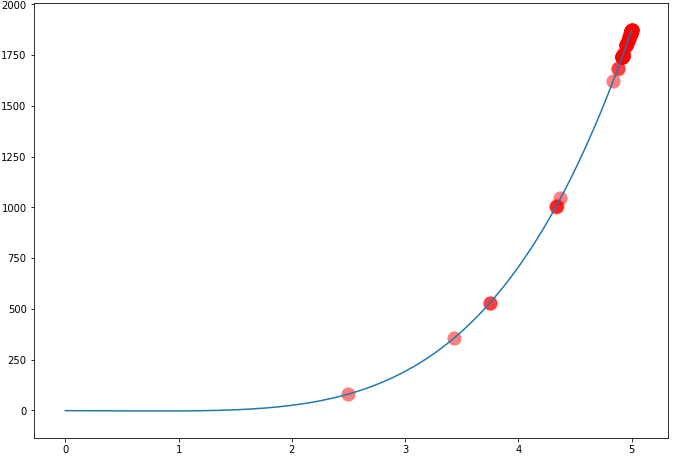
\includegraphics[width=\textwidth]{Image1.PNG}
%        \caption{Workers evolution}\label{fig:image-1}
%    \end{subfigure}
%    \\
%    \begin{subfigure}[b]{0.9\textwidth}
%        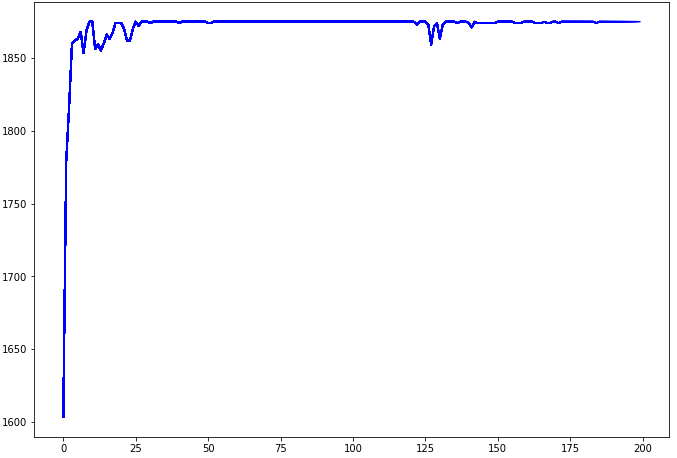
\includegraphics[width=\textwidth]{Image2.PNG}
%        \caption{Objective evolution}\label{fig:image-2}
%    \end{subfigure}
%    \caption{Optimal result with(x, y(x))max: (4.9982, 1872.1397)}
%    \label{fig:GA-result}
%\end{figure}

\end{document}

